
\documentclass{standalone}
\usepackage{xcolor}
\usepackage{pgfplots}
\pgfplotsset{compat=1.18}

\begin{document}

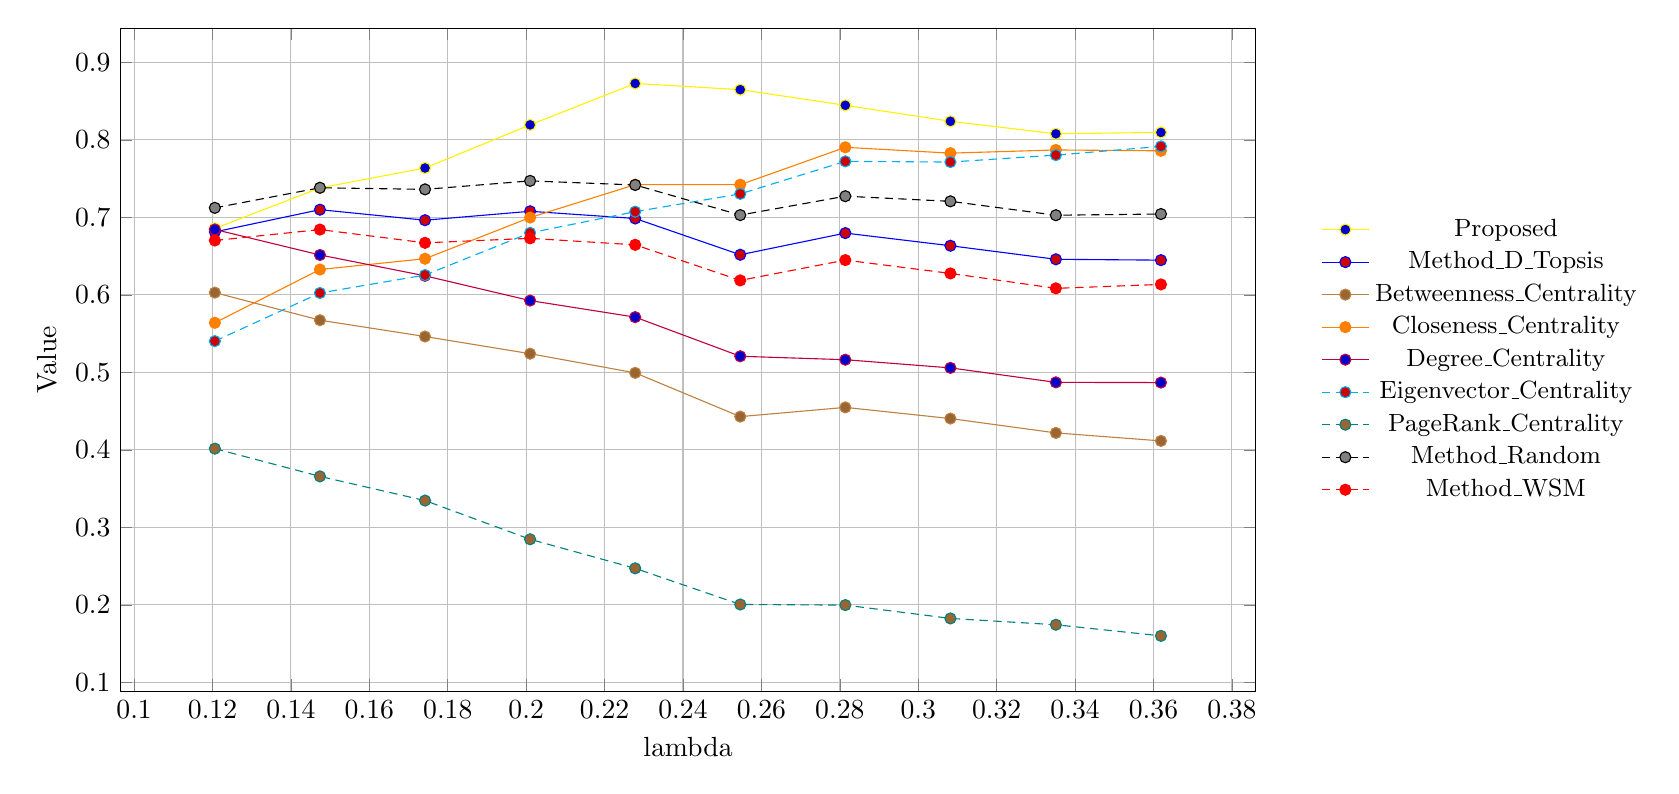
\begin{tikzpicture}
\begin{axis}[
    width=16cm,
    height=10cm,
    xlabel={lambda},
    ylabel={Value},
    grid=major,
    legend style={
        at={(1.05,0.5)},
        anchor=west,
        font=\small,
        draw=none,
        cells={align=left},
    },
]
% Proposed
\addplot+[color=yellow, mark=*] coordinates {
(0.1206,0.6857369328428025) (0.1474,0.7380520583419505) (0.1742,0.7637443962359671) (0.201,0.8194311075195474) (0.2278,0.872843596555827) (0.2546,0.8648650527737166) (0.2814,0.8446591334245239) (0.3082,0.824020204767933) (0.3351,0.8079034223234123) (0.3619,0.8096597341110718) };
\addlegendentry{Proposed}

% Method\_D\_Topsis
\addplot+[color=blue, mark=*] coordinates {
(0.1206,0.6813043266334773) (0.1474,0.7099706487818919) (0.1742,0.6963936211249927) (0.201,0.7078869522151912) (0.2278,0.6986133240202324) (0.2546,0.651809299279914) (0.2814,0.6797602687814955) (0.3082,0.6634389644694155) (0.3351,0.6459439682804652) (0.3619,0.6448412984814204) };
\addlegendentry{Method\_D\_Topsis}

% Betweenness\_Centrality
\addplot+[color=brown, mark=*] coordinates {
(0.1206,0.6029543787340671) (0.1474,0.5673359446512848) (0.1742,0.5462833240144414) (0.201,0.5241363605795287) (0.2278,0.4993847213409521) (0.2546,0.4429353827941264) (0.2814,0.4548212850462386) (0.3082,0.4404213279928034) (0.3351,0.4218996022357974) (0.3619,0.4115762378539814) };
\addlegendentry{Betweenness\_Centrality}

% Closeness\_Centrality
\addplot+[color=orange, mark=*] coordinates {
(0.1206,0.5639773644760656) (0.1474,0.6327808806452283) (0.1742,0.6466629304263464) (0.201,0.6998186721624584) (0.2278,0.7422453172698762) (0.2546,0.7422213722399192) (0.2814,0.7904320412553006) (0.3082,0.7829272410870013) (0.3351,0.7870347123513536) (0.3619,0.7859311863946075) };
\addlegendentry{Closeness\_Centrality}

% Degree\_Centrality
\addplot+[color=purple, mark=*] coordinates {
(0.1206,0.6844063901365901) (0.1474,0.6515170096110384) (0.1742,0.6246064561411008) (0.201,0.5926642345880158) (0.2278,0.5712947802144634) (0.2546,0.5208100314943364) (0.2814,0.5163566592868797) (0.3082,0.505818768281025) (0.3351,0.4871213391470056) (0.3619,0.4868511664686101) };
\addlegendentry{Degree\_Centrality}

% Eigenvector\_Centrality
\addplot+[color=cyan, mark=*] coordinates {
(0.1206,0.5403375297019927) (0.1474,0.6024550296101292) (0.1742,0.6256082756666728) (0.201,0.6800557545884104) (0.2278,0.7074168556815197) (0.2546,0.7303445319570001) (0.2814,0.77232258694699) (0.3082,0.7714409401582377) (0.3351,0.7803921611991199) (0.3619,0.7916319240404515) };
\addlegendentry{Eigenvector\_Centrality}

% PageRank\_Centrality
\addplot+[color=teal, mark=*] coordinates {
(0.1206,0.4015962279819567) (0.1474,0.3658078630598949) (0.1742,0.33458653979628) (0.201,0.2846437129847661) (0.2278,0.2471325260022776) (0.2546,0.2005083598758421) (0.2814,0.1996929976523895) (0.3082,0.1825008852717202) (0.3351,0.1743265177939858) (0.3619,0.1600013298589554) };
\addlegendentry{PageRank\_Centrality}

% Method\_Random
\addplot+[color=black, mark=*] coordinates {
(0.1206,0.712323552281462) (0.1474,0.7382506934062448) (0.1742,0.7361788440064877) (0.201,0.7471345830747429) (0.2278,0.7418388860889799) (0.2546,0.7029924564623858) (0.2814,0.7273586007206241) (0.3082,0.7207462498049821) (0.3351,0.7028157588432628) (0.3619,0.7043584713901122) };
\addlegendentry{Method\_Random}

% Method\_WSM
\addplot+[color=red, mark=*] coordinates {
(0.1206,0.6702153890255105) (0.1474,0.6842983934019979) (0.1742,0.6671835931655078) (0.201,0.6730004461484413) (0.2278,0.6646100206387167) (0.2546,0.6187001239016591) (0.2814,0.6449120784935409) (0.3082,0.627708541515943) (0.3351,0.6084531951129407) (0.3619,0.613525476188547) };
\addlegendentry{Method\_WSM}


\end{axis}
\end{tikzpicture}

\end{document}
